%
% File acl2014.tex
%
% Contact: giovanni.colavizza@epfl.ch
%%
%% Based on the style files for ACL-2013, which were, in turn,
%% Based on the style files for ACL-2012, which were, in turn,
%% based on the style files for ACL-2011, which were, in turn, 
%% based on the style files for ACL-2010, which were, in turn, 
%% based on the style files for ACL-IJCNLP-2009, which were, in turn,
%% based on the style files for EACL-2009 and IJCNLP-2008...

%% Based on the style files for EACL 2006 by 
%%e.agirre@ehu.es or Sergi.Balari@uab.es
%% and that of ACL 08 by Joakim Nivre and Noah Smith

\documentclass[11pt]{article}
\usepackage{acl2014}
\usepackage{times}
\usepackage{url}
\usepackage{latexsym}
\usepackage{graphicx}
\usepackage{subfigure}
\usepackage[font=small,skip=0pt]{caption}
%\setlength\titlebox{5cm}

% You can expand the titlebox if you need extra space
% to show all the authors. Please do not make the titlebox
% smaller than 5cm (the original size); we will check this
% in the camera-ready version and ask you to change it back.


\title{1000 years of battles}

\author{Marguerite Delcourt\\
  {\small \tt marguerite.delcourt@epfl.ch} \\
  \And
  David Froelicher\\
  {\small \tt david.froelicher@epfl.ch}\\
  \And
Christian Mouchet\\
{\small \tt christian.mouchet@epfl.ch} \\}

\date{}

\begin{document}
\maketitle

\begin{abstract}
Battles around the world and among centuries have engaged more than 209 millions of people and made more than 62 millions of casualties. Nowadays, only 10 countries are considered to be completely in peace. Even though the remaining countries are not all in an active war state, battles inside and among nations are an important matter today and have a major impact in human history. By collecting, formatting, observing and processing data from the open source and collaborative Wikipedia platform, we are able to better understand how the history of battles evolved among centuries and locations. In this report, we study more than 7,000 battles data in order to observe how battles evolved in terms of duration and number of casualties. We also notice that while the outcome of a battle can be of different types (decisive or strategic victory), the victory of a combatant mainly depends on the casualties that it suffers.
\end{abstract}


\section{Introduction}
In 1943, the soviets won the Battle of Stalingrad against the nazis while loosing 800,000 soldiers, twice the number of german casualties. In spite of these heavy losses, this soviet victory is considered as a major strategic turning point that lead to the soviet victory against the nazis' invasion. Human history contains numerous examples such as this one that show the importance and complexity of battles.

While battle-related casualties are far from being representative of all the damages caused by war, they have the particularity of being the result of a strategic and tactical planning, and are therefore worth analyzing. In this work, we make a first step towards understanding the evolution of the way powers wage battle by studying the trends and relationships between multiple battle-related features such as the initial strengths, the number of casualties or the result type of a battle. 

In order to support these observations, we first describe how we collected and processed data on more than 7,000 battles from the English Wikipedia database dump\footnote{https://meta.wikimedia.org/wiki/Data\_dumps} and provide a short spatial and temporal descriptive analysis of the resulting dataset. Then, we report on our findings by observing trends in duration, number of casualties and how indecisive the battles tends to become over the last thousand years. We isolate the adversary losses as a critical feature determining probability of victory and show that this is interestingly not the case for longer-term victories. Lastly, we compute cumulative time spent in battle for each of our extracted belligerents and provide a ranking of the most warlike ones.  


\section{Related works}
The Uppsala University has a Conflict Data Program\cite{UCDP} which is the oldest and principal provider of war related data. It is considered as the global reference in terms of armed conflicts studies. Even though this ongoing project operates at a much larger scale, their results correlate with ours (mostly for peak values). The main difference lies in a finer granularity of considering "violent events", which include but are not limited to battles, resulting in differences in trends.

Another interesting related work is the "War and Peace" article from the \textit{ourworldindata.com} website\cite{warandpeace}. Their conclusions agree with ours to state that the past was not more peaceful than the contemporary era. Their data also show that the common belief that we live in the most dangerous times is the mere consequence of our human tendency to give less importance to past conflicts than present times ones.

%ref1: http://pcr.uu.se/digitalAssets/667/c_667494-l_1-k_battle-related-deaths-by-type-of-conflict--1989-2016.pdf
%ref2: https://ourworldindata.org/war-and-peace/

\section{Data Collection}
Given the semi-structured nature of our base dataset, data collection was a significant part of our work. The task was to extract clean and normalized features for each battle related page in the English Wikipedia dump file ($\sim $44 GB). Based on the assumption that the data collection would certainly be an iterative process, we split our pipeline in three steps, enabling each of them to be ran separately and avoiding larger scale computation to be required at each iteration.

\subsection{Page extraction}
The first pipeline step is the only one to be run on the cluster. It performs the page selection based on a regular expression matching of the page title, and outputs a consolidated JSON file containing all pages. By avoiding to process any further at this step, we effectively reduced our dependency on the cluster, the output being already small enough for local processing ($\sim $123 MB, 27k pages, which was way beyond our initial estimate of 10k).

\subsection{Field extraction}
We leverage on the presence of an \textit{infobox} in most of the battle-related pages. This step looks for it in the page's source code, which is written using the Wikitext\cite{wikitext} markup language. The syntax generating the \textit{infobox} template\cite{template} provides a \textit{key}-\textit{value} set for each battle where the keys are conveniently standardized (e.g. \textit{date}, \textit{combatant1}, \textit{combatant2}, \dots).   Values, however, are free text field, usually containing Wikitext, and natural language formatted for humans. For this reason we qualified our dataset of being semi-structured. The output of this part is a file containing one JSON per battle, with its extracted \textit{key}-\textit{value} set, thus reducing the size to $\sim $14 MB. The number of pages where an \textit{infobox} could be found was 7486, closer to our initial estimate, and still comfortably large. It appeared that many pages were in fact redirects, drafts or discussion pages.  

Using this representation, a preliminary analysis was performed to pinpoint potential features that could be extracted from the fields.

[TABLE OF FIELDS]

\section{Descriptive Analysis}
While providing exhaustive descriptive analysis for every feature is not feasible within this short report, given their diversity, the reader can refer to the companion notebook. In this section, we focus on analyzing the spatio-temporal coverage of our dataset, as it is important for the rest of the discussion.

\begin{figure}[h]
	\centering
	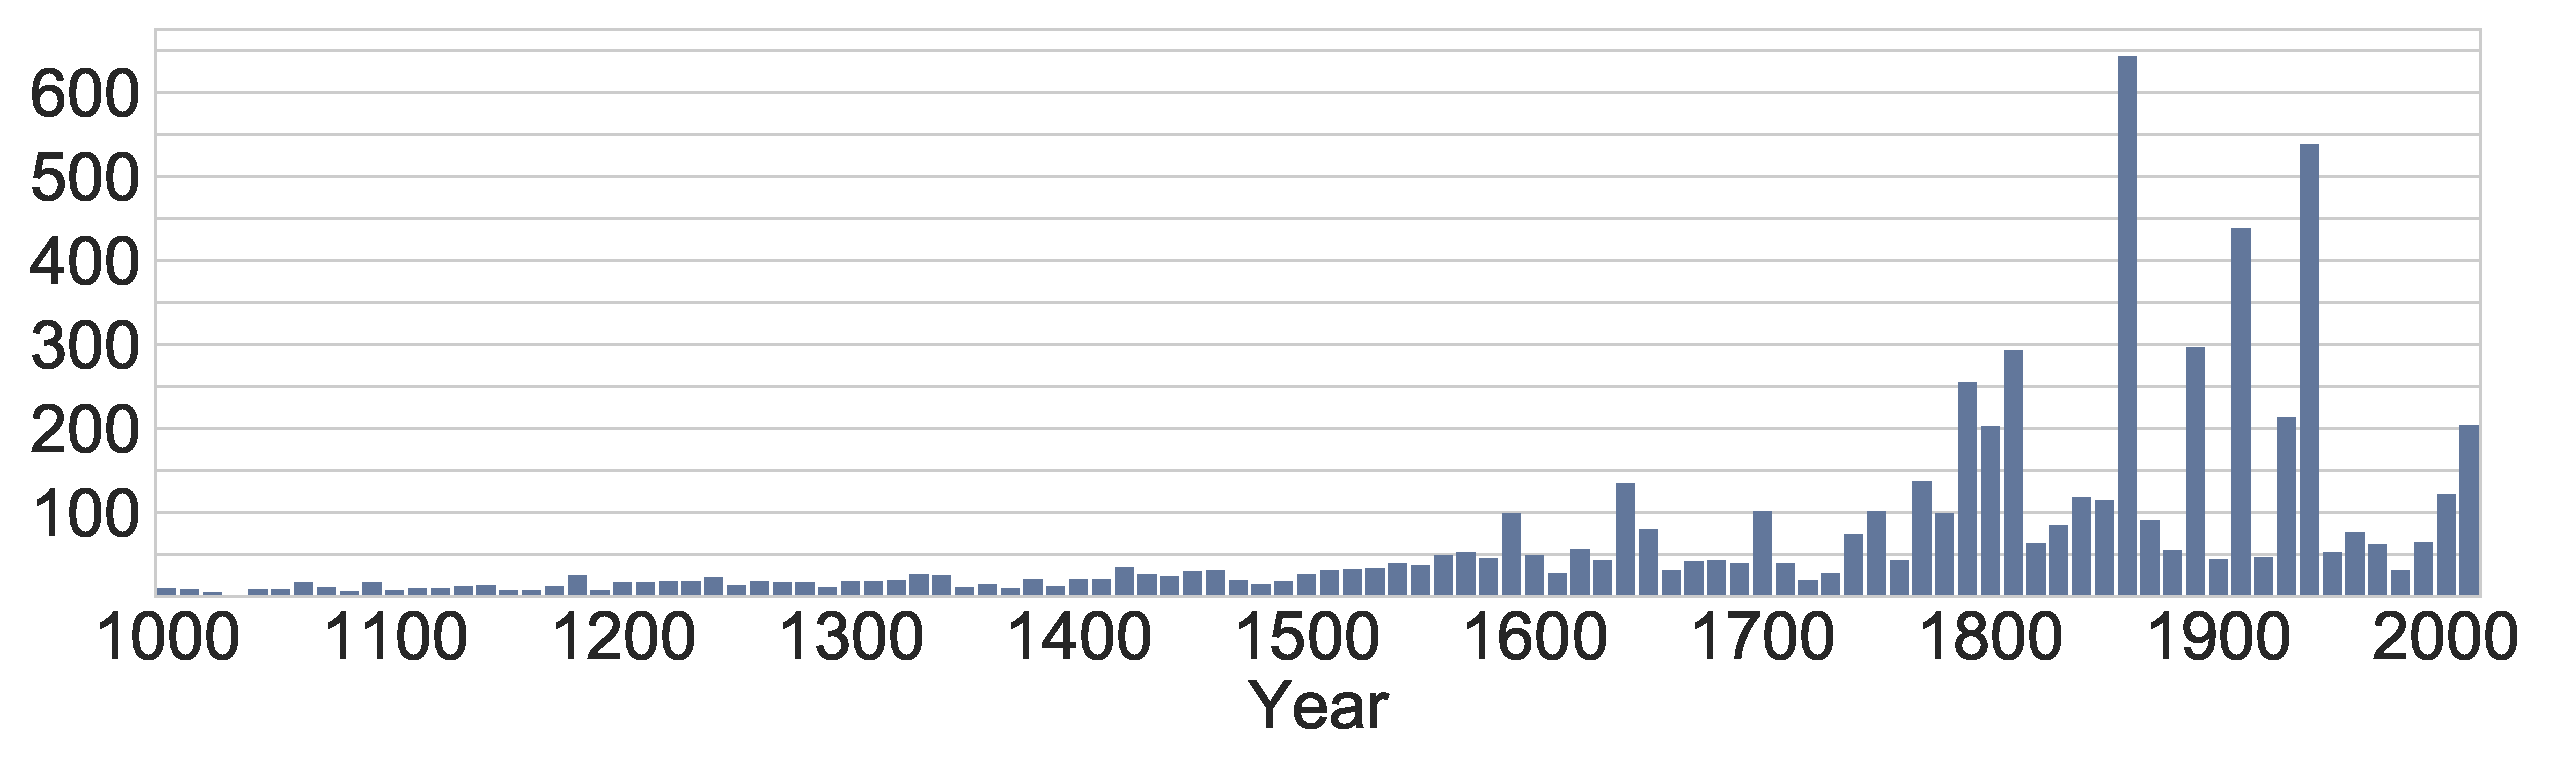
\includegraphics[width=\linewidth]{figures/temporal_coverage.eps}
	\caption{Battle count per decade}
	\label{temporal_coverage}
\end{figure}

\section{Exploratory Analysis}
\input{sections/exploratory_analysis.tex}

\section{Results}
In this Section, we report on our analysis of the dataset we built, focusing on the most interesting findings. The interested reader will find our data exploration and extended analysis in the companion notebook.

\subsection{Duration of the Battles}

We observe that the duration of the battles over the last millennium increased almost monotonically. In fact, we can see in Figure \ref{fig:durThByCent} that the average duration of a battle has never been higher than nowadays. We show here the duration in order of magnitude. This is because the distribution of the duration values was concentrated on small values with a heavy tail going to extreme values. Thus, using the average of the logarithm duration values, we attenuate the influence of extreme values while showing an augmentation of almost one order of magnitude in the battles' duration. Notice that the average duration of a battle was almost 34 days during the XX$^{th}$ century while it is currently of 64 days in the XXI$^{st}$ century.

 \begin{figure}[h]
	\centering	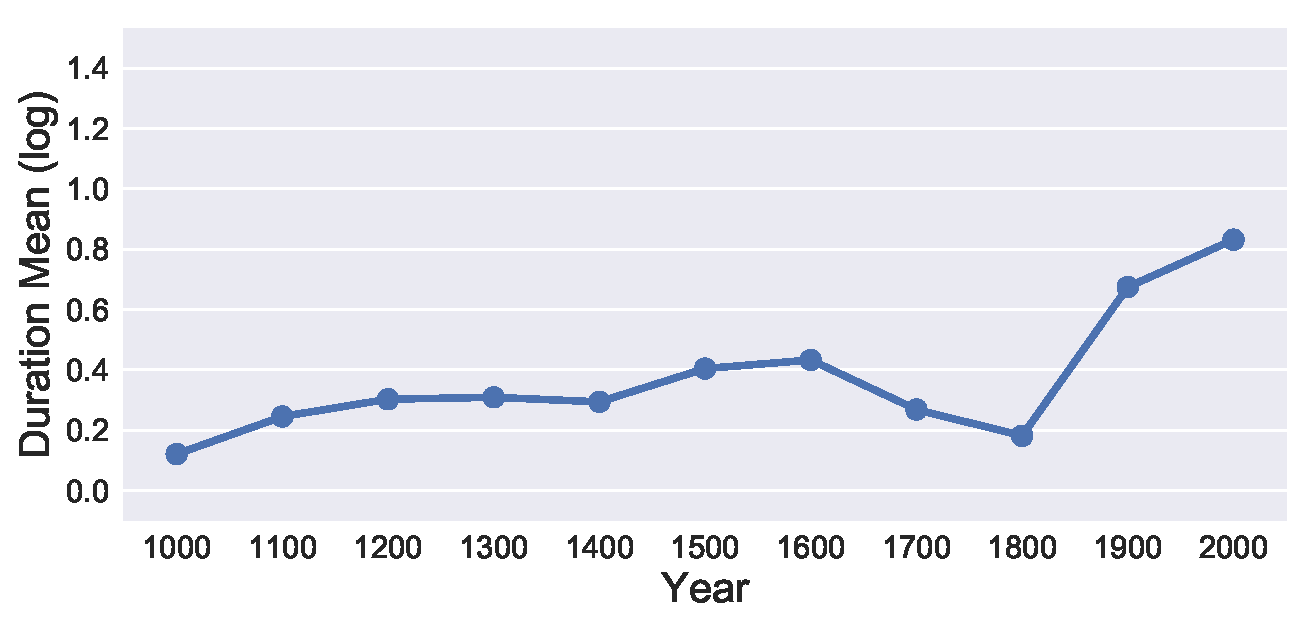
\includegraphics[width=\linewidth]{figures/durThByCent}
	\caption{Mean of the duration of battles in the last thousand years by century on a logarithmic scale.}\label{fig:durThByCent}
	\centering
\end{figure}

\subsection{Evolution of the Casualties}

In Figure \ref{fig:casuPerCent}, we notice that the percentage of soldiers engaged in a battle that are wounded, killed, captured or that disappeared decreases throughout the years. We observe that, following the same trend as shown in Figure \ref{fig:durThByCent} for the battle's duration, the percentage of casualties decreased before increasing in the XX$^{th}$ century. We can infer that in both cases this is due to the world wars because they contain numerous battles which made countless casualties, notably because of technology advances such as aerial forces or gaz attacks.
 \begin{figure}[h]
	\centering	\includegraphics[width=\linewidth]{figures/casuPerCent}
	\caption{Mean of the percentage of casualties in the soldiers.}\label{fig:casuPerCent}
	\centering
\end{figure}

\subsection{Indecisiveness of the Battles}

We observe, in Figure \ref{fig:IndecBattles}, that battles tend to be more indecisive nowadays than they were in the past. In fact, the fraction of indecisive battle within one century is increasing slowly since year 1200 and at a much higher rate over the last two centuries. This can be explained by two factors: the first being that battles in the further past were most likely reported by the winner with probably less accuracy and objectiveness than they are now. The second explanation lies in operational theaters (like cities) and tactics enabled by modern weaponry such as long range weapons. Ultimately, longer distances between the combatants and modern combat vehicles greatly enhanced the ability to retreat.

 \begin{figure}[h]
	\centering	\includegraphics[width=\linewidth]{figures/indThByCent}
	\caption{Mean of the percentage of indecisive battles over the last thousand year.}\label{fig:IndecBattles}
	\centering
\end{figure}

From Figures \ref{fig:durThByCent}, \ref{fig:casuPerCent} and \ref{fig:IndecBattles}, we conclude that battles are longer, make less casualties and are more indecisive over the years. This supports the fact that nowadays the battle's purpose is not only to invade another territory by beating the other combatant. In fact, modern battles seem to be more complex in the sense that they often serve a higher strategic or even political goal and have their result studied in many different axis.

\subsection{Outcome of the battles}

We continue our analysis by studying the advantage provided to a combatant that has fewer of casualties, larger strengths  and  lower casualties to strength ratio. We compute the percentage of battles won by a combatant that had at least one of these advantages, grouped by three different victory types: \textit{tactical}, \textit{strategic},  \textit{decisive}. The \textit{tactical} level is the lower one in the military level of planning\footnote{http://www.esquire.com/news-politics/politics/news/a39985/four-levels-of-war/}. Therefore, involving narrower scope decisions and shorter-term consequences. On the other end, the \textit{strategic} level is the highest one, involving longer-term
consequences.

We first observe that an advantage in strength only is not sufficient to increase one's chances to win a battle, as this would completely disregard other tactical advantages of the opponent. On the other hand, the a-posteriori advantage in the casualties (both in ratio and absolute value) is much more significant, as it is present in around 75\% of the victories for all but strategic ones. Interestingly, we observe that for this victory type, an advantage in absolute casualties has much less effect on the outcome (in fact, it looks like it is the opposite), and a little less effect in the ratio advantage. This would typically generalize the mentioned case of the Battle for Stalingrad, where the Nazis' strategy was not able to provide victory even though it was tactically superior. Figure \ref{fig:victoryAdvantage} illustrates these observations.

 \begin{figure}[h]
	\centering	\includegraphics[width=\linewidth]{figures/VictoryAdvantage}
	\caption{Victory percentage with advantage in either strength, casualties or casualty ratio.}\label{fig:victoryAdvantage}
	\centering
\end{figure}

\subsection{Years of Battles per Countries}
In Figure \ref{fig:FightingDurationRanking}, we observe that among all countries in our dataset, France is the one that fought the most. Nevertheless, the United States, which are a major actor in the international history of battles, were only created in 1776 when they proclaimed their independence. Thus, it is interesting to do the same ranking starting from this year. 
 \begin{figure}[h]
 	\centering
 	\begin{subfigure}[b]{0.475\linewidth}
 		\centering
 		\includegraphics[width=\linewidth]{figures/YearsFightingRanking.eps}
 		\caption[]%
 		{{\small 1000 --- 1700}}    
 		\label{fig:FightingDurationRankingOld}
 	\end{subfigure}
 	\begin{subfigure}[b]{0.475\linewidth}  
 		\centering 
 		\includegraphics[width=\linewidth]{figures/YearsFightingRankingModern}
 		\caption[]%
 		{{\small 1701 --- 1900}}    
 		\label{fig:FightingDurationRankingModern}
 	\end{subfigure}
 	\vskip0.2\baselineskip
	\caption{Cumulated duration of battles engagement per country. From 100 in (a) and from 1776 and the United States independence in (b).} 
 	\label{fig:FightingDurationRanking}
 \end{figure}
 
 These results tend to support the common belief that the United States are always in war. In fact, as we observe in Figure \ref{fig:USAFightingTimeline}, they were engaged in a at least one battle per year for more than 150 years in 242 years of existence.
 \begin{figure}[h]
 	\centering	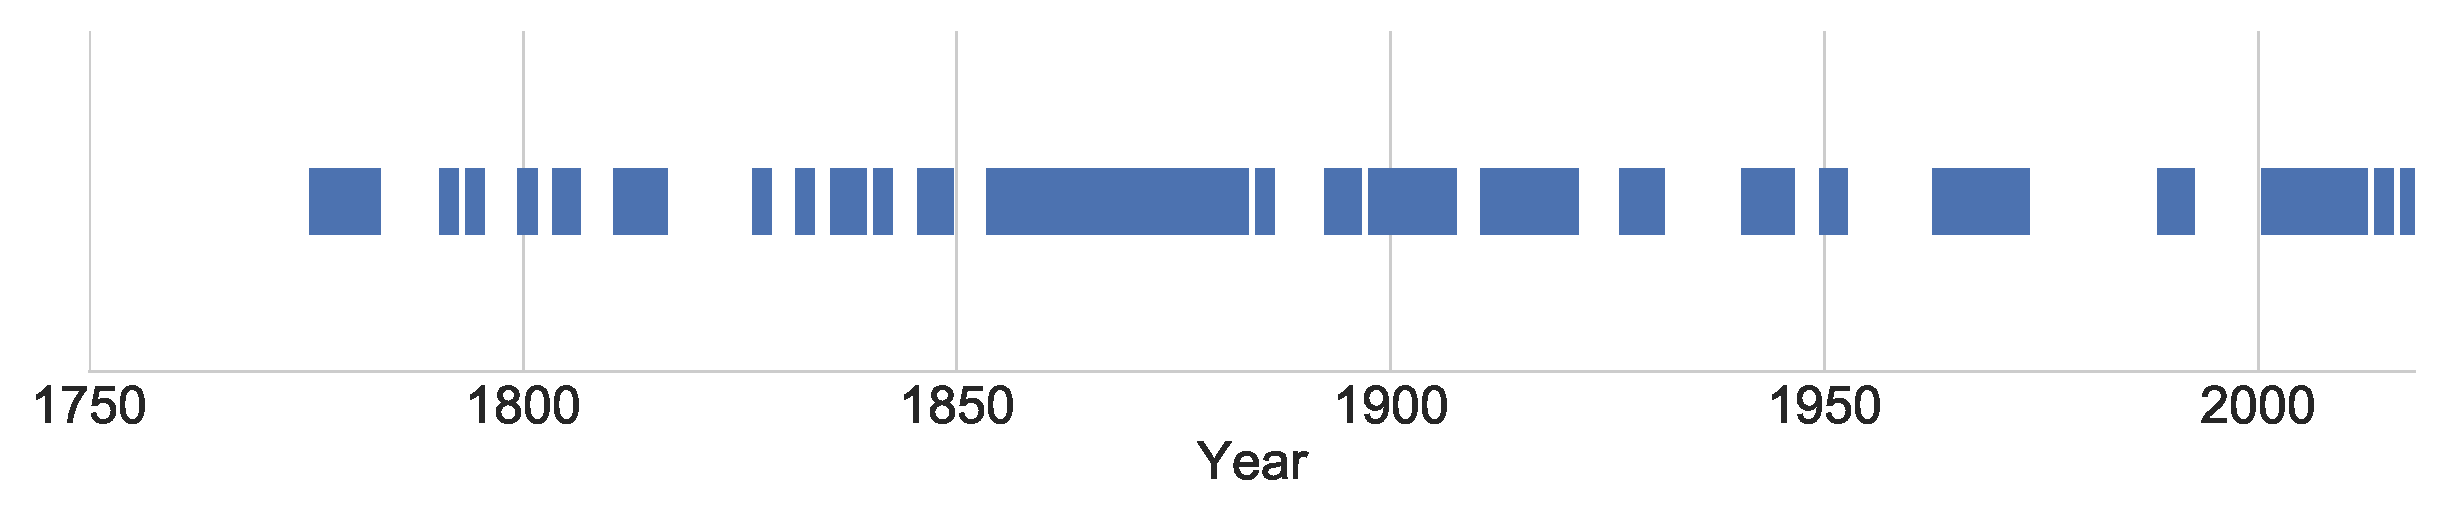
\includegraphics[width=\linewidth]{figures/USAFighting}
 	\caption{Timeline of the USA engagement in battles.}\label{fig:USAFightingTimeline}
 	\centering
 \end{figure}



\section{Conclusion}
In this report, we have collected and processed the data from Wikipedia in order to retrieve useful information about battles through the human history. We have focused on the battles after year 1000 and observe interesting patterns that shown that while the battles are becoming lengthier and more complex, they are also making less casualties on the battle fields. In fact, we study the number of casualties among soldiers and we expect that the number of civilian casualties is higher in modern battles. This can be an interesting study for futur work. We have also noticed that the number of casualties is determinant for the victory of a battle. In fact, a combatant suffering less casualties has almost 80\% of chances to win. 

\end{document}
